Для начала попробуем установить Wi-Fi соединение и подсоединиться к RPi без Ethernet-соединения. 

\begin{figure}[h!]
\center{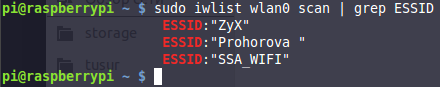
\includegraphics[width=0.6\linewidth]{mm_1}}
\caption{ просканировали сеть }
\label{mm_1:mm_1}
\end{figure}


\begin{figure}[h!]
\center{
\includegraphics[width=0.6\linewidth]{mm_2}}
\caption{ путь к config }
\label{mm_2:mm_2}
\end{figure}


\begin{figure}[h!]
\center{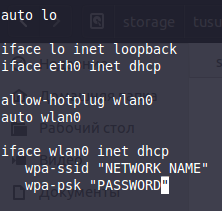
\includegraphics[width=0.3\linewidth]{mm_3}}
\caption{ config }
\label{mm_3:mm_3}
\end{figure}


\begin{figure}[h!]
\center{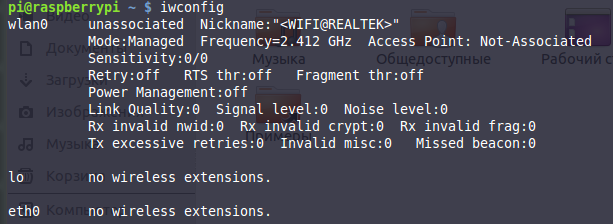
\includegraphics[width=0.7\linewidth]{mm_4}}
\caption{ config }
\label{mm_4:mm_4}
\end{figure}

подняли сетку в режиме Managed

\begin{figure}[h!]
\center{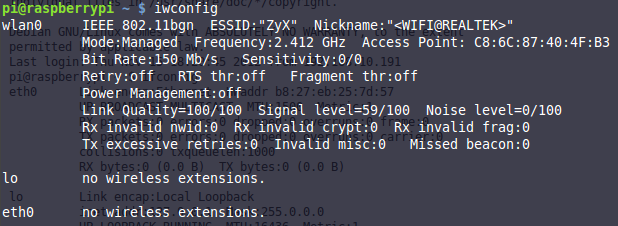
\includegraphics[width=0.7\linewidth]{mm_5}}
\caption{ config }
\label{mm_5:mm_5}
\end{figure}


тут можно рассказать про разные режимы даптеров (их 6) и про мониторящий режим. Устройство может в определенный момент времени находиться только в одном режиме.

Настроим адаптер в режим приема пакетов. Для этого необходимо ввести команду 
sudo iwconfig wlan0 mode monitor
При попытке ввести данную команду видим следующее сообщение:


\begin{figure}[h!]
\center{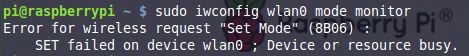
\includegraphics[width=0.6\linewidth]{mm_6}}
\caption{ ресурс занят }
\label{mm_6:mm_6}
\end{figure}

это связано с тем, что в системе работает network interface plugging daemon (ссылка на распберри пи орг)
необходимо его отключить для того, чтобы перевести устройство в другой режим работы

напишем небольшой bash-скрипт, который будет переводить адаптер в режим перехвата пакетов и содержать следующие команды:
sudo service ifplugd stop #останавливаем работу демона
sudo ifconfig wlan0 down #отключаем wi-fi соединение
sudo iwconfig wlan0 mode monitor #включаем прослушивающий режим
sudo ifconfig wlan0 up #включаем wi-fi соединение
sudo service ifplugd start #запускаем демона
iwconfig #проверям настройки

результат работы скрипта приведен на рисунке ... Устройство теперь в режиме перехвата пакетов. Данный скрипт необходимо запускать снова при перезапуске системы, поскольку по умолчанию устройство переходит в режим managed 

\begin{figure}[h!]
\center{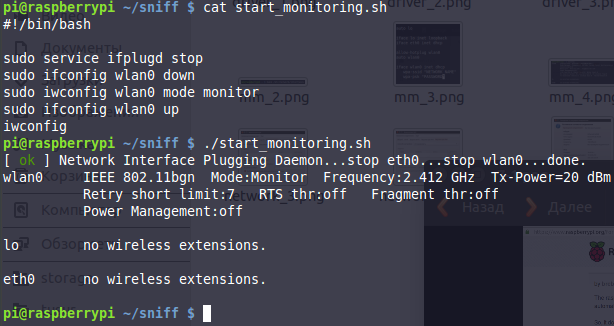
\includegraphics[width=0.6\linewidth]{mm_7}}
\caption{ результат выполнения скрипта }
\label{mm_7:mm_7}
\end{figure}

\clearpage







